\documentclass[tikz,border=3pt]{standalone}
\usepackage[T1]{fontenc}
\usepackage{amsmath}
\usepackage{XCharter}
\usepackage[xcharter]{newtxmath}
\usepackage[scaled=.92]{helvet}
\usepackage{pgfplots}
\usetikzlibrary{arrows.meta,positioning,fit,calc,backgrounds,decorations.pathreplacing,patterns}
\usepgfplotslibrary{groupplots,fillbetween}
\pgfplotsset{compat=1.18}
\definecolor{ink}{HTML}{172536}
\definecolor{rgb}{HTML}{3563B8}
\definecolor{event}{HTML}{17857C}
\definecolor{fusion}{HTML}{76529C}
\definecolor{reference}{HTML}{8994A3}
\definecolor{warn}{HTML}{AC5948}
\definecolor{muted}{HTML}{657183}
\definecolor{rule}{HTML}{D9E0E8}
\definecolor{pale}{HTML}{F5F7FA}
\color{ink}
\tikzset{box/.style={rounded corners=2pt,draw=rule,fill=white,align=center,inner sep=4pt,font=\sffamily\fontsize{9}{10.8}\selectfont,minimum height=9mm},rb/.style={box,draw=rgb!50,fill=rgb!5},eb/.style={box,draw=event!50,fill=event!5},fb/.style={box,draw=fusion!55,fill=fusion!5},arrow/.style={-{Latex[length=1.8mm]},line width=.65pt,draw=muted},note/.style={font=\sffamily\fontsize{8.4}{10.2}\selectfont,align=center,text=muted},heading/.style={font=\sffamily\fontsize{10}{12}\selectfont\bfseries,align=left,text=ink}}
\pgfplotsset{paper/.style={width=15.7cm,height=6cm,axis lines*=left,axis line style={rule},tick style={draw=none},tick label style={font=\sffamily\fontsize{8.8}{10.4}\selectfont,text=muted},label style={font=\sffamily\fontsize{9.4}{11}\selectfont,text=ink},title style={font=\sffamily\fontsize{10}{12}\selectfont\bfseries,text=ink},legend style={draw=none,fill=none,font=\sffamily\fontsize{9}{11}\selectfont,cells={anchor=west}},grid=major,grid style={rule!65,line width=.3pt},minor tick num=0,scaled ticks=false,unbounded coords=jump,clip mode=individual}}
\begin{document}

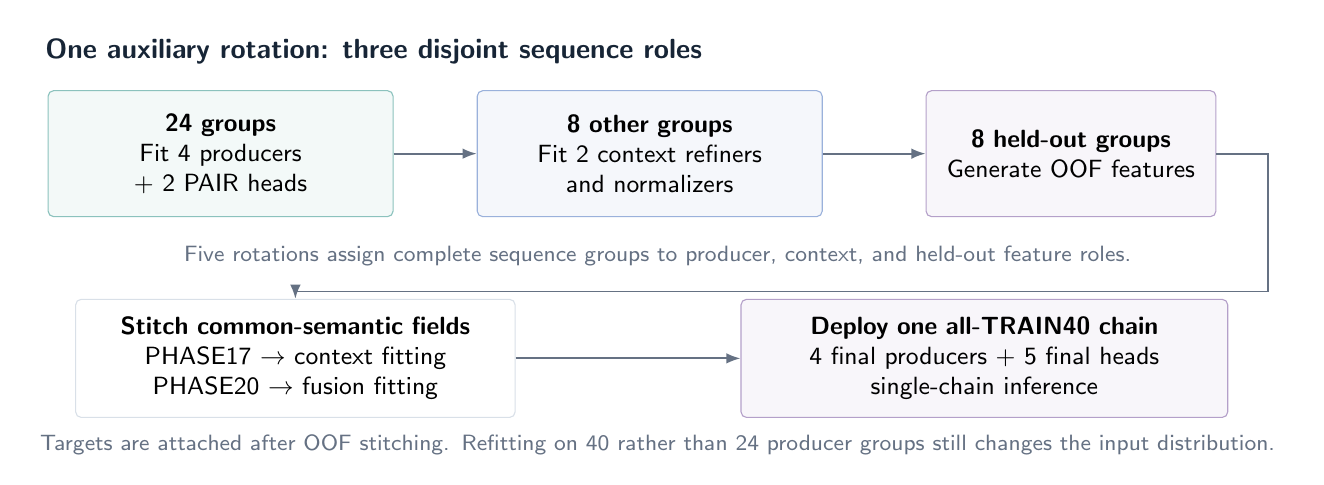
\begin{tikzpicture}[x=1cm,y=1cm]
\path[use as bounding box] (0,-.25) rectangle (16.1,5.2);
\node[heading,anchor=west] at (.1,4.9) {One auxiliary rotation: three disjoint sequence roles};
\node[eb,text width=4.1cm,minimum height=16mm] (p) at (2.45,3.6) {\textbf{24 groups}\\Fit 4 producers + 2 PAIR heads};
\node[rb,text width=4.1cm,minimum height=16mm] (h) at (7.9,3.6) {\textbf{8 other groups}\\Fit 2 context refiners\\and normalizers};
\node[fb,text width=3.4cm,minimum height=16mm] (v) at (13.25,3.6) {\textbf{8 held-out groups}\\Generate OOF features};
\draw[arrow] (p)--(h);\draw[arrow] (h)--(v);
\node[note,text width=14.5cm] at (8,2.3) {Five rotations assign complete sequence groups to producer, context, and held-out feature roles.};
\node[box,text width=5.3cm,minimum height=15mm] (st) at (3.4,1.0) {\textbf{Stitch common-semantic fields}\\PHASE17 \(\to\) context fitting\\PHASE20 \(\to\) fusion fitting};
\node[fb,text width=5.9cm,minimum height=15mm] (dep) at (12.15,1.0) {\textbf{Deploy one all-TRAIN40 chain}\\4 final producers + 5 final heads\\single-chain inference};
\draw[arrow] (v.east)--++(.65,0)--++(0,-1.75)-|(st.north);
\draw[arrow] (st)--(dep);
\node[note,text width=16cm] at (8,-.1) {Targets are attached after OOF stitching. Refitting on 40 rather than 24 producer groups still changes the input distribution.};
\end{tikzpicture}
\end{document}
